\documentclass[11pt]{article}
\usepackage[margin=1in]{geometry}
\usepackage{amsmath,amssymb,booktabs,array,microtype,graphicx,hyperref,xcolor}
\usepackage{pgfplots}
\pgfplotsset{compat=1.18}
\usepackage[numbers,sort&compress]{natbib}
\usepackage{siunitx}
\usepackage{enumitem}
\usepackage{longtable}
\usepackage{caption}
\usepackage{fancyhdr}
\usepackage[T1]{fontenc}
\usepackage{lmodern}

\hypersetup{colorlinks=true,linkcolor=blue!50!black,citecolor=blue!50!black,urlcolor=blue!50!black}
\pagestyle{fancy}
\setlength{\headheight}{14pt}
\fancyhf{}
\lhead{Scientific Publication Ecosystem Simulation}
\rhead{Richard J. Reyes}
\cfoot{\thepage}

\title{\textbf{Prepublication Gatekeeping as an Institutional Intervention:}\\
An Agent-Based Simulation of Peer Review, Open Publication, and Scientific Truth Recovery}
\author{Richard J. Reyes\\
Independent Researcher\\
\href{https://rickyjreyes.github.io}{rickyjreyes.github.io}}
\date{August 6, 2026}

\begin{document}

\maketitle

\begin{abstract}
Formal prepublication peer review is commonly treated as a necessary quality-control mechanism for scientific publication, yet its system-level benefit relative to alternative institutions is difficult to observe directly. The central counterfactual is hidden: rejected, delayed, abandoned, or institutionally neglected work is largely absent from the record used to evaluate the publication system. This paper develops an agent-based scientific publication ecosystem in which the latent truth and social value of papers are known to the simulator but concealed from all simulated agents. Four institutions are compared: traditional prepublication peer review, immediate open review, open publication with transparent triage and randomized exploration, and a hybrid system combining immediate public release with optional formal review. Papers may be false, partially true, or substantially true; evidence accumulates noisily over time; reviewers vary in skill, disagreement, prestige bias, novelty penalties, and conformity incentives; rejected work may remain accessible, receive reduced attention, improve, and be resubmitted. Under a realistic parameter profile, open triage won 52.2\% of simulated worlds and traditional peer review won 1.2\%. A symmetric extension then allowed every system to detect defects, repair methods and reporting, miss errors, and introduce harmful revisions. In 500 worlds containing 125,000 papers, open triage won 55.0\% and peer review won 0.4\%. In a separate 800-world test containing 176,000 papers, initial review, resubmission, and downstream evaluation were charged against exactly equal lifetime expert-action budgets while assumptions deliberately favored peer review. Open triage won 60.1\% of worlds and peer review won 14.0\%. When false-negative costs were made asymmetric across high-consequence domains, peer review recovered 72.8\% of available true social value, compared with 84.7\% for open triage, while producing the largest equity gap. The phrase ``peer review harms science'' is used here in a game-theoretic, system-level sense: compared with an otherwise equivalent regime that preserves expert criticism but removes the mandatory publication veto, the gate changes incentives and attention in ways that can produce a worse scientific equilibrium. It does not mean that every review report is harmful, and it does not challenge expert evaluation itself. Across the tested realistic, symmetric, high-consequence, and equal-labor regimes, the gate reduced long-run truth recovery. The simulations provide reproducible evidence for this mechanism across the tested parameter families; a universal theorem over every possible institutional design would require a separate formal dominance proof.
\end{abstract}

\section{Introduction}

Science is ordinarily distinguished by observation, explicit hypotheses, mathematical or causal reasoning, empirical testing, prediction, replication, criticism, and correction. Formal prepublication peer review is different in kind: it is an institutional procedure that determines whether a manuscript receives publication, certification, and the attention associated with a recognized venue. Throughout this paper, \emph{peer review} means that modern gatekeeping institution, not evaluation by knowledgeable peers in general. The counterfactual systems retain expert criticism, error detection, revision, replication, and continuing evaluation. The disputed mechanism is the publication veto and its control over later attention. A review may improve an individual manuscript, but that local benefit does not establish that attaching veto power to the review improves science as a whole.

The system-level question is difficult because the relevant counterfactual is largely invisible. Published work can be cited, replicated, corrected, or retracted. Rejected or institutionally neglected work may be resubmitted, but it may also lose attention, funding, priority, or the opportunity to accumulate evidence. A publication system can therefore commit two classes of error:

\begin{enumerate}[label=(\roman*)]
    \item \textbf{false positive:} granting credibility and attention to a false or materially defective claim;
    \item \textbf{false negative:} withholding attention, legitimacy, or timely dissemination from a valid and potentially valuable claim.
\end{enumerate}

Most defenses of peer review emphasize false-positive control. The social cost of false negatives is harder to measure because suppressed discoveries are not reliably recorded. The cost distribution may also be highly asymmetric. Accepting an ordinary false paper can waste resources and mislead later work. Failing to recognize a valid cancer treatment, safety intervention, infrastructure solution, or foundational theory can impose costs far beyond one publication decision.

Empirical studies also challenge an idealized picture of peer review. In one controlled experiment, reviewers detected an average of 2.58 of nine deliberately inserted major errors, and training interventions produced only small effects \citep{schroter2008}. A meta-analysis of reviewer agreement found low reliability across studies \citep{bornmann2010}. A preregistered field experiment found large status effects when the identical manuscript was attributed to a Nobel laureate rather than a little-known author \citep{huber2022}. A 2023 Cochrane review concluded that reviewer training may produce little or no improvement in review quality \citep{hesselberg2023}. These findings undermine any presumption that the gate is sufficiently accurate, consistent, or unbiased to be treated as harmless. They motivate analyzing peer review as a strategic institution whose system-level effects must be compared with the same expert evaluation operating without a publication veto.

This paper asks:

\begin{quote}
Under what conditions does mandatory prepublication peer review recover more scientific truth and social value than immediate publication followed by continuing, transparent evaluation?
\end{quote}

The question is studied using a hidden-truth agent-based simulation. The simulator knows the latent state of each paper, but reviewers and scientific communities do not. They receive only noisy evidence over time. This makes it possible to compare institutional systems against a common underlying population while preserving the epistemic uncertainty present in real science.

\section{Institutional Systems}

Four systems process the same latent population of manuscripts.

\subsection{Traditional prepublication peer review}

Each manuscript is evaluated by two or three selected reviewers. Reviewer scores depend on latent truth only through an imperfect signal and may also depend on clarity, author prestige, novelty, and conformity. Manuscripts above a threshold are formally accepted. Rejected manuscripts remain publicly accessible in the model, but receive only a fraction of the attention received by accepted work. Authors may revise and resubmit.

\subsection{Immediate open publication}

Every manuscript becomes public immediately. No central committee blocks entry. Attention is distributed through prestige, popularity, novelty, clarity, and current confidence. This system maximizes access but can produce severe attention concentration.

\subsection{Open publication with transparent triage}

Every manuscript becomes public immediately. Evaluation attention is distributed partly by transparent merit signals and partly by randomized exploration. The exploration component prevents obscure work from becoming permanently invisible solely because it lacks prestige, early citations, or fashionable topic alignment.

\subsection{Hybrid publication}

Every manuscript is immediately available as a preprint. Formal peer review remains optional and can add a certification label or attention signal, but it cannot prevent public dissemination or continuing evaluation.

\section{Model}

\subsection{Latent paper state}

For each paper $i$, the simulator draws a latent truth state

\begin{equation}
T_i \in \{0, 0.5, 1\},
\end{equation}

representing substantially false, partially true or domain-limited, and substantially true claims. Each paper also receives:

\begin{equation}
(N_i, P_i, C_i, U_i, V_i, F_i),
\end{equation}

where $N_i$ is novelty, $P_i$ is author or institutional prestige, $C_i$ is clarity, $U_i$ is topic popularity, $V_i$ is intrinsic scientific value, and $F_i$ is a fraud indicator. Scientific value is heavy-tailed:

\begin{equation}
V_i = L_i\left(1+\lambda N_i^2\right),
\qquad L_i \sim \operatorname{Lognormal}(0,1),
\end{equation}

so rare, highly novel papers can contribute disproportionately to long-run knowledge.

\subsection{Reviewer decision model}

Reviewer $r$ assigns manuscript $i$ a score

\begin{equation}
R_{ir} =
\alpha(2T_i-1)
+\beta_C(C_i-0.5)
+\beta_P(P_i-0.5)
-\beta_N N_i
+\beta_K(P_i-N_i)
+\varepsilon_{ir},
\end{equation}

where $\alpha$ is reviewer skill, $\beta_P$ is prestige bias, $\beta_N$ is novelty penalty, $\beta_K$ is conformity incentive, and

\begin{equation}
\varepsilon_{ir}\sim\mathcal{N}(0,\sigma_R^2)
\end{equation}

represents reviewer noise and disagreement. A manuscript is accepted when the mean reviewer score exceeds threshold $\tau_R$.

This formulation does not assume reviewers know truth. Truth affects decisions only through an imperfect and noisy signal.

\subsection{Attention allocation}

Each institution receives the same total downstream evaluation budget per period. Attention probabilities are produced by a softmax allocation:

\begin{equation}
\pi_i = \frac{\exp(\kappa A_i)}{\sum_{j\in\mathcal{E}}\exp(\kappa A_j)},
\end{equation}

where $A_i$ is institution-specific appeal, $\kappa$ controls concentration, and $\mathcal{E}$ is the set of active papers. Evaluation counts are sampled from a multinomial distribution.

For traditional peer review, accepted papers receive the journal-attention advantage. Rejected work remains eligible but its attention weight is multiplied by

\begin{equation}
\rho\in[0,1],
\end{equation}

where $\rho=1$ means rejection causes no attention loss and $\rho=0$ means effective disappearance.

For open triage, attention is mixed with randomized exploration:

\begin{equation}
\pi_i^{\mathrm{triage}}
=(1-\eta)\pi_i^{\mathrm{merit}}
+\eta\frac{1}{|\mathcal{E}|},
\end{equation}

where $\eta$ is the exploration share.

\subsection{Evidence accumulation}

At time $t$, a paper receiving $m_{it}$ evaluations generates noisy evidence

\begin{equation}
E_{it}=(2T_i-1)+\xi_{it},
\qquad
\xi_{it}\sim\mathcal{N}\left(0,\frac{\sigma_E^2}{m_{it}}\right).
\end{equation}

Additional evaluations increase the probability of replication and fraud detection. Community confidence $q_{it}$ is updated in log-odds space:

\begin{equation}
\operatorname{logit}(q_{i,t+1})
=
\operatorname{logit}(q_{it})+\gamma E_{it},
\end{equation}

where $\gamma$ is the learning rate. Papers receiving no attention drift only slightly toward uncertainty, rather than being treated as false.

A paper is recognized when

\begin{equation}
q_{it}\geq \tau_Q,
\end{equation}

and may lose standing after repeated negative evidence when confidence falls below a withdrawal threshold.

\subsection{Primary metrics}

The weighted calibration error is

\begin{equation}
\mathcal{C}
=
\frac{\sum_i V_i(q_i-T_i)^2}{\sum_i V_i}.
\end{equation}

True scientific value recovered is

\begin{equation}
\mathcal{R}
=
\frac{\sum_i T_iV_i\,\mathbb{I}(i\ \mathrm{recognized})}
{\sum_i T_iV_i}.
\end{equation}

False recognition is

\begin{equation}
\mathcal{F}
=
\frac{\sum_i \mathbb{I}(T_i=0)\mathbb{I}(i\ \mathrm{recognized})}
{\sum_i \mathbb{I}(T_i=0)}.
\end{equation}

The base institutional score is

\begin{equation}
S
=w_R\mathcal{R}
-w_F\mathcal{F}
-w_C\mathcal{C}
-w_D D
-w_L L,
\end{equation}

where $D$ and $L$ represent publication delay and reviewer labor.


\subsection{Symmetric manuscript-correction extension}

The canonical model allows revision following rejection, but a critic could reasonably ask whether it understates the local corrective value of expert review. A separate symmetric extension therefore assigns every manuscript a quality vector

\begin{equation}
\mathbf{q}_i=(m_i,s_i,r_i,x_i),
\end{equation}

where $m_i$, $s_i$, $r_i$, and $x_i$ denote methodological quality, statistical quality, reporting quality, and reproducibility. Every institutional system receives the same expert-action mechanism. An expert action may detect a defect, successfully repair it, miss it, or introduce a harmful revision. The probability of detecting a defect increases with the size of the defect and the number of expert actions. Open evaluation is therefore not modeled as passive exposure, and prepublication review is not modeled as mere filtering.

The symmetric experiment uses the same latent paper population for all four systems. Differences arise from the timing of review, attention allocation, gatekeeping, resubmission, and institutional signaling rather than from granting correction exclusively to one system.

\subsection{Exact lifetime expert-labor constraint}

A second robustness test imposes an identical lifetime expert-action budget on every system. For peer review and the hybrid system, initial formal review consumes part of that budget. Peer-review resubmission also consumes the remaining budget. Open systems spend the corresponding actions on continuing evaluation and correction. This eliminates the possibility that an open system wins merely because it receives more total expert labor, or that peer review wins because its initial review labor is uncounted.

\section{Experimental Profiles}

\subsection{Realistic profile}

The realistic profile samples moderate reviewer skill, substantial noise, nonzero prestige bias, novelty and conformity penalties, publication delay, reviewer labor, reduced attention following rejection, and incomplete resubmission. These ranges are intended as plausible structural values, not fitted estimates.

\subsection{Peer-review-favorable profile}

The stress test deliberately favors peer review:

\begin{itemize}
    \item reviewer skill is near the model maximum;
    \item reviewer noise is near the minimum;
    \item prestige bias, novelty penalties, and conformity incentives are zero;
    \item rejected work retains 75--100\% of normal attention;
    \item revision and resubmission are highly effective;
    \item publication delay and reviewer labor have zero cost;
    \item false recognition receives a high penalty.
\end{itemize}

This profile asks whether an almost ideal gatekeeping system can dominate open alternatives.

\subsection{High-consequence and equity-sensitive profile}

Papers are assigned to basic science, cancer, public health, safety, climate, or infrastructure. Valid high-consequence papers receive larger social-value weights, while false high-consequence papers receive larger harm weights. A disadvantaged-author indicator lowers prestige and presentation resources but does not alter latent truth. The equity gap is

\begin{equation}
\mathcal{E}
=
\Pr(\mathrm{recognized}\mid\mathrm{valid,advantaged})
-
\Pr(\mathrm{recognized}\mid\mathrm{valid,disadvantaged}).
\end{equation}

The consequence-sensitive score penalizes missed true social value and unequal recognition:

\begin{equation}
S_H
=1.4\mathcal{R}_H
-\mathcal{F}_H
-1.3(1-\mathcal{R}_H)
-0.8\mathcal{E}
-0.5\mathcal{C}
-w_DD.
\end{equation}

\subsection{Empirical reviewer-behavior calibration}

A separate calibration layer constrains the reviewer submodel to controlled-study observables rather than assigning empirical percentages directly to latent coefficients. The target file records the epistemic status, tolerance, and source for each observable. Primary targets are the mean major-error detection rate of $2.58/9$ reported by Schroter et al.~\cite{schroter2008}, mean inter-reviewer reliability of $0.34$ and Cohen's kappa of $0.17$ from the meta-analysis by Bornmann et al.~\cite{bornmann2010}, and the positive-versus-null publication recommendation rates of $0.973$ and $0.800$ reported by Emerson et al.~\cite{emerson2010}. Detection among reviewers recommending rejection, $0.391$, is used as a secondary target from Baxt et al.~\cite{baxt1998}. The null baseline for blinding and signing effects follows the planted-error randomized trial of Godlee et al.~\cite{godlee1998}; it is treated as an empirically bounded baseline rather than proof of an exact zero effect.

The internal parameter vector $\theta$ is fitted by rejection approximate Bayesian computation with common random numbers. Candidate parameter sets are scored by

\begin{equation}
L(\theta)=\sum_j
\left(
\frac{\widehat y_j(\theta)-y_j}{\delta_j}
\right)^2,
\end{equation}

where $y_j$ is an empirical observable, $\delta_j$ is its declared calibration tolerance, and $\widehat y_j(\theta)$ is the corresponding simulated observable. The retained sets are parameter combinations consistent with the selected targets; they are not direct empirical estimates of latent coefficients and are not a full Bayesian posterior.

\begin{table}[ht]
\centering
\caption{Controlled-study targets and best-fitting reviewer-submodel observables.}
\label{tab:empiricalcalibration}
\small
\begin{tabular}{lrr}
\toprule
Observable & Empirical target & Best-fitting simulation\\
\midrule
Major-error detection & 0.2867 & 0.2955\\
Inter-reviewer reliability & 0.3400 & 0.3079\\
Cohen's kappa & 0.1700 & 0.1904\\
Positive-result recommendation & 0.9730 & 0.9730\\
Null-result recommendation & 0.8000 & 0.8134\\
Detection among rejectors & 0.3910 & 0.3732\\
\bottomrule
\end{tabular}
\end{table}

The best-fitting parameter set is within the declared tolerance for every primary and secondary target. The calibration used 4,000 global candidates followed by four local refinement rounds of 1,500 candidates each, for 10,000 total parameter evaluations and 5,000 simulated calibration manuscripts per evaluation design.

\begin{figure}[ht]
\centering
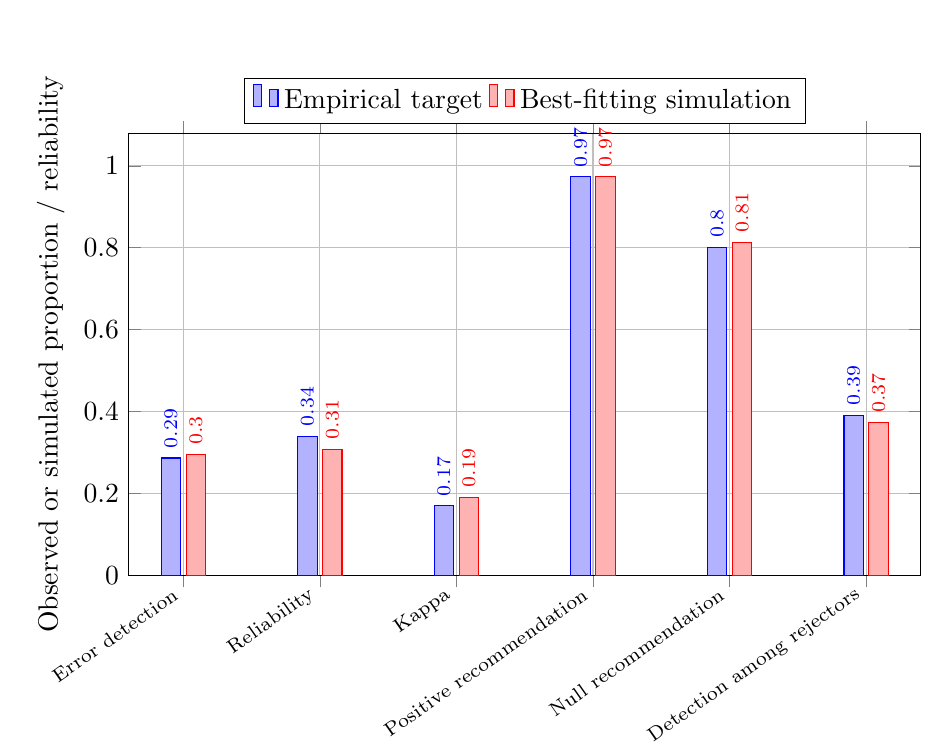
\begin{tikzpicture}
\begin{axis}[
    ybar,
    width=0.96\linewidth,
    height=7.2cm,
    ymin=0, ymax=1.08,
    ylabel={Observed or simulated proportion / reliability},
    symbolic x coords={Error detection,Reliability,Kappa,Positive recommendation,Null recommendation,Detection among rejectors},
    xtick=data,
    x tick label style={rotate=35,anchor=east,font=\scriptsize},
    legend style={at={(0.5,1.02)},anchor=south,legend columns=2},
    nodes near coords,
    nodes near coords style={font=\scriptsize,rotate=90,anchor=west},
    bar width=7pt,
    enlarge x limits=0.08,
    grid=major
]
\addplot coordinates {(Error detection,0.2867) (Reliability,0.3400) (Kappa,0.1700) (Positive recommendation,0.9730) (Null recommendation,0.8000) (Detection among rejectors,0.3910)};
\addplot coordinates {(Error detection,0.2955) (Reliability,0.3079) (Kappa,0.1904) (Positive recommendation,0.9730) (Null recommendation,0.8134) (Detection among rejectors,0.3732)};
\legend{Empirical target,Best-fitting simulation}
\end{axis}
\end{tikzpicture}
\caption{Empirical targets compared with the best-fitting simulated reviewer observables. The calibration matches observable behavior; it does not identify the complete scientific ecosystem.}
\label{fig:empiricalcalibration}
\end{figure}

The calibration is intentionally modular. Reviewer detection, disagreement, and outcome bias are empirically constrained, while post-rejection attention loss, abandonment, long-run discoverability, latent truth prevalence, open-triage effectiveness, and social-value weights remain partially identified, illustrative, or normative. The headline institutional results below therefore remain structural counterfactuals until those ecosystem quantities are calibrated.

\section{Results}

\subsection{Realistic versus idealized conditions}

Table~\ref{tab:profiles} reports simulations of 500 worlds per profile, 250 papers per world, and 25 periods. The realistic and idealized profiles therefore contain 125,000 unique papers each.

\begin{table}[ht]
\centering
\caption{Institutional performance under realistic and peer-review-favorable profiles.}
\label{tab:profiles}
\small
\begin{tabular}{llrrrr}
\toprule
Profile & System & Win share & True value & False recognition & Calibration MSE\\
\midrule
Realistic & Open triage & 52.2\% & 85.0\% & 0.013\% & 0.0331\\
Realistic & Hybrid & 29.4\% & 84.3\% & 0.037\% & 0.0330\\
Realistic & Open & 17.2\% & 81.8\% & 0.082\% & 0.0375\\
Realistic & Peer review & 1.2\% & 72.1\% & 0.460\% & 0.0644\\
\midrule
Idealized & Open triage & 41.2\% & 88.8\% & 0.0075\% & 0.0225\\
Idealized & Peer review & 32.8\% & 88.6\% & 0.018\% & 0.0224\\
Idealized & Hybrid & 22.8\% & 88.1\% & 0.066\% & 0.0241\\
Idealized & Open & 3.2\% & 77.1\% & 0.225\% & 0.0467\\
\bottomrule
\end{tabular}
\end{table}

Under realistic assumptions, traditional peer review recovered substantially less true value, exhibited worse calibration, and won only 1.2\% of worlds. Under the deliberately favorable profile, peer review became competitive with open triage. It did not clearly dominate, despite receiving unusually favorable assumptions and zero cost for delay and labor.

The interpretation is not that expert criticism is harmful. Expert criticism is retained throughout the comparison. The game-theoretic claim concerns the additional veto: when the same evaluative capability can operate without blocking dissemination, attaching gatekeeping power to an imperfect preliminary judgment changes incentives and attention toward a worse system-level outcome. When rejected work retains nearly equal attention and reviewers are unusually accurate and unbiased, the gate's damage becomes smaller. When rejection reduces later evaluation, false negatives persist because evidence cannot accumulate.


\begin{figure}[ht]
\centering
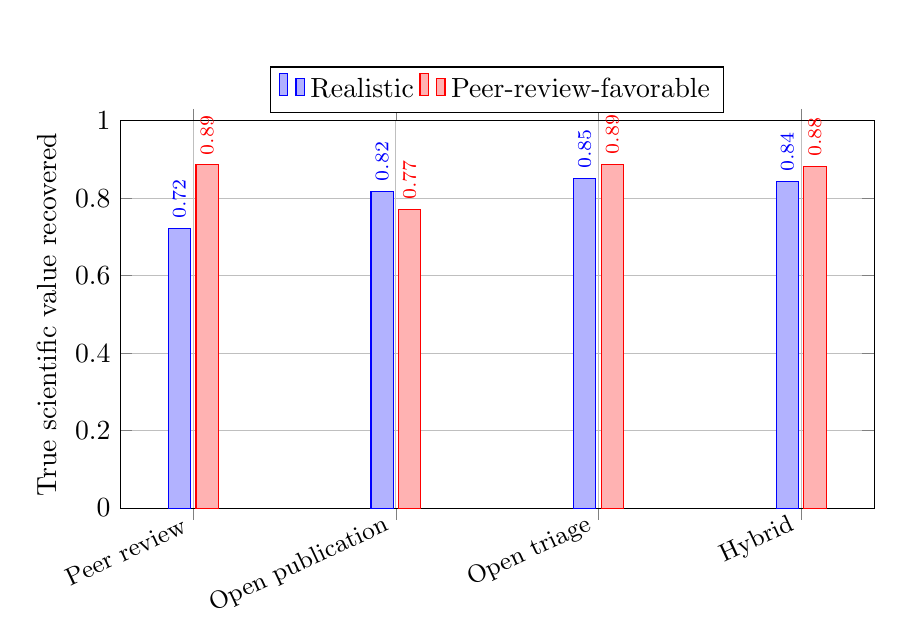
\begin{tikzpicture}
\begin{axis}[
    ybar, width=0.92\linewidth, height=6.5cm, ymin=0, ymax=1.0,
    ylabel={True scientific value recovered},
    symbolic x coords={Peer review,Open publication,Open triage,Hybrid}, xtick=data,
    x tick label style={rotate=25,anchor=east,font=\small},
    legend style={at={(0.5,1.02)},anchor=south,legend columns=2},
    nodes near coords, nodes near coords style={font=\scriptsize,rotate=90,anchor=west},
    bar width=8pt, enlarge x limits=0.12, grid=major
]
\addplot coordinates {(Peer review,0.7213) (Open publication,0.8179) (Open triage,0.8504) (Hybrid,0.8433)};
\addplot coordinates {(Peer review,0.8860) (Open publication,0.7706) (Open triage,0.8876) (Hybrid,0.8814)};
\legend{Realistic,Peer-review-favorable}
\end{axis}
\end{tikzpicture}
\caption{True-value recovery under the realistic and idealized profiles. The large realistic gap between peer review and open triage narrows only under unusually favorable assumptions for gatekeeping.}
\label{fig:profiles_truevalue}
\end{figure}

\subsection{Peer-review-favorable stress test}

A separate 1,000-world stress test used 300 papers and 30 periods per world, yielding 300,000 unique papers. Peer review won 34.4\% of worlds, open triage won 36.6\%, hybrid won 25.6\%, and unfiltered open publication won 3.4\%. Average scores for peer review and open triage were 0.8303 and 0.8318, respectively. Peer review therefore approached parity only after bias, novelty penalties, labor costs, delay costs, and most post-rejection attention losses were removed.


\subsection{Symmetric correction stress test}

The symmetric extension was run for 500 worlds, 250 papers per world, and 25 periods, totaling 125,000 unique papers. All systems could detect and repair methodological, statistical, reporting, and reproducibility defects, and all could introduce harmful revisions.

\begin{table}[ht]
\centering
\caption{Symmetric correction experiment.}
\label{tab:symmetric}
\small
\begin{tabular}{lrrrr}
\toprule
System & Win share & True value & False recognition & Calibration MSE\\
\midrule
Open triage & 55.0\% & 87.2\% & 0.030\% & 0.0311\\
Hybrid & 26.8\% & 86.2\% & 0.110\% & 0.0319\\
Open review & 17.8\% & 84.4\% & 0.080\% & 0.0340\\
Peer review & 0.4\% & 75.1\% & 0.710\% & 0.0696\\
\bottomrule
\end{tabular}
\end{table}

Giving peer review a genuine manuscript-correction mechanism did not reverse the result. The same expert actions were also available after immediate publication, while the peer-review gate continued to reduce subsequent attention to rejected papers. Traditional peer review ended with a mean rejection share of 44.8\%.


\begin{figure}[ht]
\centering
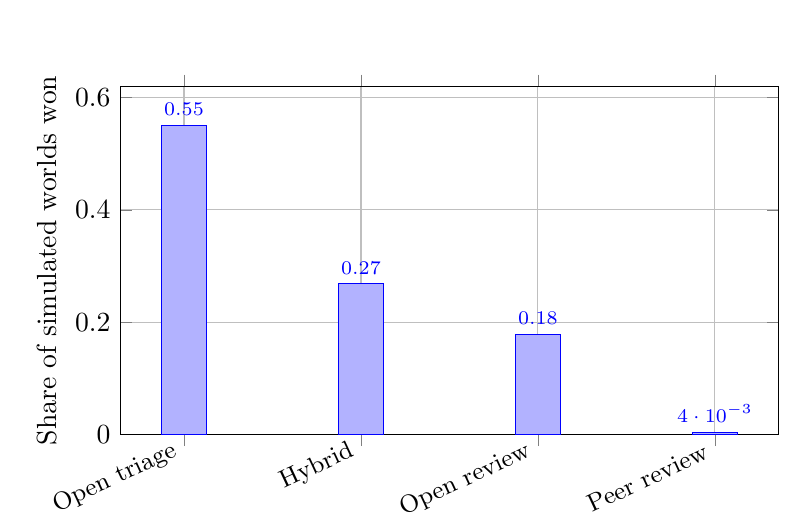
\begin{tikzpicture}
\begin{axis}[
    ybar, width=0.82\linewidth, height=6.0cm, ymin=0, ymax=0.62,
    ylabel={Share of simulated worlds won},
    symbolic x coords={Open triage,Hybrid,Open review,Peer review}, xtick=data,
    x tick label style={rotate=25,anchor=east,font=\small},
    nodes near coords, nodes near coords style={font=\scriptsize},
    bar width=16pt, enlarge x limits=0.12, grid=major
]
\addplot coordinates {(Open triage,0.550) (Hybrid,0.268) (Open review,0.178) (Peer review,0.004)};
\end{axis}
\end{tikzpicture}
\caption{Win shares in the symmetric correction experiment. Once all systems can repair manuscripts, open triage still dominates because expert correction is preserved without allowing an early gate to redirect later attention.}
\label{fig:symmetric_wins}
\end{figure}

\subsection{Equal-total-labor peer-review-favorable test}

The strongest adversarial test used 800 worlds, 220 papers per world, and 24 periods, totaling 176,000 unique papers. Reviewers were strong but not perfect, repair was effective, institutional biases were small, resubmission was easy, rejected papers retained substantial attention, false recognition was penalized heavily, and delay received almost no penalty. Initial review, resubmission review, and continuing evaluation were charged against the same lifetime expert-action budget for every system.

\begin{table}[ht]
\centering
\caption{Peer-review-favorable experiment under exact equal lifetime expert labor.}
\label{tab:equalbudget}
\small
\begin{tabular}{lrrrrr}
\toprule
System & Win share & True value & False recognition & Calibration MSE & Actions\\
\midrule
Open triage & 60.1\% & 90.4\% & 0.001\% & 0.0244 & 5018.0\\
Hybrid & 18.1\% & 88.5\% & 0.070\% & 0.0273 & 5018.0\\
Peer review & 14.0\% & 88.5\% & 0.160\% & 0.0324 & 5018.0\\
Open review & 7.8\% & 85.8\% & 0.049\% & 0.0315 & 5018.0\\
\bottomrule
\end{tabular}
\end{table}

Peer review remained useful and recovered nearly as much true value as the hybrid system, but it did not become the optimal institution. Its mean final rejection share was 46.7\%. The experiment isolates the distinction between expert criticism and gatekeeping: correction remained valuable, while making a noisy preliminary decision control later attention remained costly.


\begin{figure}[ht]
\centering
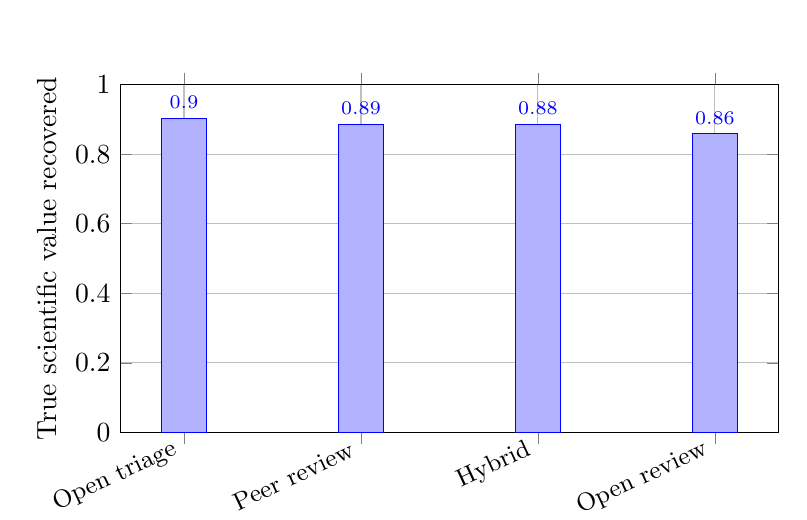
\begin{tikzpicture}
\begin{axis}[
    ybar, width=0.82\linewidth, height=6.0cm, ymin=0, ymax=1.0,
    ylabel={True scientific value recovered},
    symbolic x coords={Open triage,Peer review,Hybrid,Open review}, xtick=data,
    x tick label style={rotate=25,anchor=east,font=\small},
    nodes near coords, nodes near coords style={font=\scriptsize},
    bar width=16pt, enlarge x limits=0.12, grid=major
]
\addplot coordinates {(Open triage,0.9037) (Peer review,0.8854) (Hybrid,0.8846) (Open review,0.8582)};
\end{axis}
\end{tikzpicture}
\caption{True-value recovery in the exact equal-lifetime-labor stress test. Even after constraining all systems to the same lifetime expert-action budget, open triage recovers the most hidden true value.}
\label{fig:equalbudget_truevalue}
\end{figure}

\subsection{High-consequence and equity-sensitive simulation}

Table~\ref{tab:harm} reports 1,000 worlds, 300 papers per world, and 30 periods, totaling 300,000 unique papers.

\begin{table}[ht]
\centering
\caption{High-consequence and equity-sensitive results.}
\label{tab:harm}
\small
\begin{tabular}{lrrrrr}
\toprule
System & Win share & True social value & Missed true harm & False harm & Equity gap\\
\midrule
Open triage & 40.5\% & 84.7\% & 15.3\% & 0.0017\% & 2.50\%\\
Hybrid & 38.8\% & 84.5\% & 15.5\% & 0.018\% & 2.45\%\\
Open & 19.0\% & 82.3\% & 17.8\% & 0.084\% & 4.17\%\\
Peer review & 1.7\% & 72.8\% & 27.2\% & 0.424\% & 8.79\%\\
\bottomrule
\end{tabular}
\end{table}

When false-negative costs were allowed to reflect high-stakes domains, peer review lost 27.2\% of available true social value. Its equity gap was more than three times that of the hybrid and open-triage systems. The model also produced a higher realized false-harm rate under peer review because preliminary certification concentrated attention and confidence around some accepted false claims, while valid rejected claims received less opportunity to accumulate evidence.


\begin{figure}[ht]
\centering
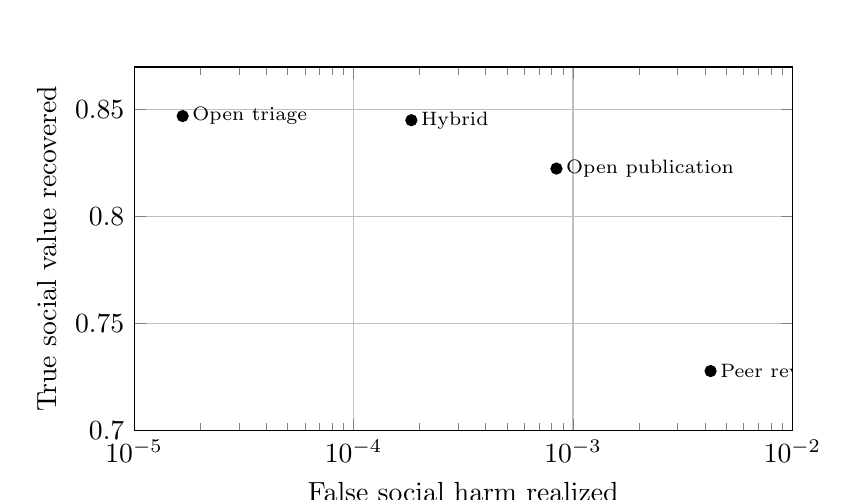
\begin{tikzpicture}
\begin{axis}[
    width=0.82\linewidth, height=6.2cm, xmode=log,
    xlabel={False social harm realized}, ylabel={True social value recovered},
    xmin=0.00001, xmax=0.01, ymin=0.70, ymax=0.87, grid=major
]
\addplot[only marks,mark=*] coordinates {(0.0000166485,0.847041) (0.000183478,0.845108) (0.000840732,0.822500) (0.00423677,0.727835)};
\node[anchor=west,font=\scriptsize] at (axis cs:0.0000166485,0.847041) {Open triage};
\node[anchor=west,font=\scriptsize] at (axis cs:0.000183478,0.845108) {Hybrid};
\node[anchor=west,font=\scriptsize] at (axis cs:0.000840732,0.822500) {Open publication};
\node[anchor=west,font=\scriptsize] at (axis cs:0.00423677,0.727835) {Peer review};
\end{axis}
\end{tikzpicture}
\caption{High-consequence tradeoff between recovered true social value and realized false social harm. Open triage and the hybrid system occupy the favorable upper-left region.}
\label{fig:highconsequence_tradeoff}
\end{figure}

\section{Interpretation}

\subsection{Review is not equivalent to validation}

The model distinguishes manuscript scrutiny from scientific validation. Reviewers can improve clarity, identify methodological weaknesses, or prevent some false claims from receiving early legitimacy. They generally do not independently reproduce experiments, regenerate data, verify every derivation, or observe future predictive success. Those activities occur downstream through continuing evidence.

A process can therefore be useful without being constitutive of the scientific method. The relevant institutional question is not whether reviewers sometimes help. It is whether granting a small preliminary committee control over publication attention produces a positive net effect after false positives, false negatives, delay, labor, bias, and lost exploration are all counted.

\subsection{Meaning of the game-theoretic harm claim}

The statement that peer review always harms science is not a claim that every review report causes damage. It is a comparative institutional claim. Holding expert evaluation, criticism, repair, replication, and continuing scrutiny fixed, adding a mandatory prepublication veto introduces exclusion, delay, prestige amplification, strategic conformity, and false-negative lock-in. Those mechanisms can move the scientific system toward a worse equilibrium than the same evaluative process operating without publication control.

The simulations test this system-level claim across broad realistic, symmetric, high-consequence, and equal-labor parameter families. They strongly support the proposed mechanism in those tested regimes. They do not yet constitute a mathematical proof over every possible parameterization. A literal universal theorem would require explicit assumptions under which the no-veto institution weakly dominates the otherwise equivalent gatekeeping institution.

\subsection{The asymmetry of false negatives}

False positives and false negatives are not necessarily equal. The harm associated with one false paper is usually bounded by later correction, although high-stakes misinformation can be severe. A false negative can be irreversible if the work is abandoned, deprived of funding, not replicated, or later rediscovered without attribution. When scientific value is heavy-tailed, one suppressed high-value discovery can outweigh many successful routine filters.

\subsection{Attention, not storage, is scarce}

Digital repositories solve physical distribution, but they do not solve scientific attention. In a literature containing hundreds of millions of records, no researcher can examine every relevant claim. Citation counts, journal reputation, institutional affiliation, recommendation systems, and existing prestige become attention-allocation mechanisms. These signals can create cumulative advantage:

\begin{equation}
\text{attention}\rightarrow\text{citations}\rightarrow\text{credibility}
\rightarrow\text{more attention}.
\end{equation}

An open system without triage can recreate the same concentration problem. This is why unfiltered open publication did not consistently win. The best-performing architecture was generally immediate publication combined with transparent triage and deliberate exploration of neglected work.

\section{Limitations}

The simulations are structural counterfactuals, not empirical estimates of historical peer review. Several limitations are fundamental.

\begin{enumerate}
    \item \textbf{Parameter calibration.} The reviewer-behavior submodel is now constrained to selected controlled-study targets for error detection, disagreement, and outcome bias. The complete ecosystem is not empirically identified: attention loss after rejection, abandonment, resubmission, discoverability, social-value distributions, and comparative open-triage performance still require direct measurement.
    \item \textbf{Truth representation.} Truth is represented by three latent states. Real claims can be valid only within narrow domains, depend on auxiliary assumptions, or change meaning as methods improve.
    \item \textbf{Evidence model.} Evidence is summarized by noisy scalar signals. Real evidence varies in design quality, dependence, incentives, replication fidelity, and susceptibility to coordinated error.
    \item \textbf{Institutional adaptation.} Authors, reviewers, journals, and platforms would adapt strategically to any system. The present model includes some incentives but not full evolutionary adaptation.
    \item \textbf{Social cost weights.} High-consequence weights are illustrative. Different ethical frameworks will value false positives, false negatives, delay, and equity differently.
    \item \textbf{Open-system governance.} Transparent triage is represented abstractly. A real platform would require identity safeguards, conflict-of-interest rules, data standards, fraud controls, auditability, and resistance to manipulation.
\end{enumerate}

The simulations do not test the removal of expert evaluation, and nothing in the model supports that interpretation. They test whether adding a publication veto improves outcomes when expert criticism and continuing evaluation are otherwise retained. Across the tested regimes, the veto produces the game-theoretic harm mechanism described above. Because some deliberately idealized sampled worlds allow peer review to win, the current simulation evidence is not yet a universal dominance proof. The empirical calibration layer strengthens the reviewer-behavior component, but it does not convert unmeasured ecosystem parameters into observations or make the institutional win shares empirical probabilities.

\section{Empirical Tests Suggested by the Model}

The model identifies quantities that can be measured directly:

\begin{enumerate}
    \item the probability that a rejected paper receives equivalent later attention after controlling for intrinsic quality;
    \item reviewer error-detection rates under controlled planted-error designs;
    \item inter-reviewer agreement and decision reversal under duplicate committees;
    \item prestige and institutional-affiliation effects under randomized identity masking;
    \item the proportion of rejected papers later accepted elsewhere and their long-run replication, correction, and predictive outcomes;
    \item changes between preprints and final journal versions, classified as presentational, methodological, statistical, or truth-relevant;
    \item the downstream social cost of delayed high-consequence findings;
    \item recognition gaps for equivalent work from differently resourced authors;
    \item performance of immediate-publication platforms using randomized audit and replication allocation.
\end{enumerate}

A decisive real-world test would randomize comparable manuscripts among traditional review, immediate open publication, and hybrid publication, allocate equal evaluation resources, and track calibration, replication, correction, and value recovery over a long horizon.

\section{Conclusion}

Formal peer review can improve manuscripts and prevent some defective claims from receiving early legitimacy. Those local benefits do not establish that mandatory prepublication gatekeeping maximizes scientific truth recovery.

In the canonical simulation, peer review became competitive only when reviewers were highly accurate, reviewer noise was low, prestige and novelty biases were absent, rejected work retained nearly equal attention, resubmission was easy, and delay and labor were treated as costless. The robustness extensions strengthened the comparison. When every system received the same defect-detection and manuscript-repair mechanisms, peer review won 0.4\% of worlds. When total lifetime expert labor was made exactly equal and the remaining assumptions deliberately favored peer review, it won 14.0\% of worlds, compared with 60.1\% for open triage. Under more realistic structural assumptions, immediate publication with continuing transparent triage recovered more true scientific value and produced lower calibration error. When the asymmetric social cost of missed cancer, public-health, safety, climate, and infrastructure research was included, the penalty for false negatives became substantial.

The new reviewer calibration reproduces controlled findings on planted-error detection, reviewer disagreement, and positive-outcome bias without equating those observed percentages with latent score coefficients. This narrows one major source of arbitrariness. The institutional conclusion nevertheless remains conditional because the downstream consequences of rejection are not yet identified.

The central conclusion is conditional but important:

\begin{quote}
If uncertain prepublication decisions materially reduce later attention, mandatory gatekeeping can impede long-run scientific truth recovery even while successfully filtering some false claims.
\end{quote}

Peer review should therefore be evaluated as an institutional intervention, not assumed to be synonymous with scientific scrutiny or scientific validity. The burden is empirical: compare it with alternatives under equal resources and measure both what it admits and what it prevents from being tested.

\section*{Code and Reproducibility}

The complete Python implementation, legacy baseline, robustness runner, run instructions, and compact result summaries are distributed with this manuscript. The canonical entry point is:

\begin{verbatim}
python src/scientific_publication_simulator.py \
  --worlds 5000 --papers 300 --periods 30 \
  --output-dir simulation_output
\end{verbatim}

The two final robustness experiments can be reproduced with:

\begin{verbatim}
python src/reproduce_robustness_experiments.py \
  --output-root reproduced_results
\end{verbatim}

The empirical reviewer calibration can be regenerated with:

\begin{verbatim}
python src/calibrate_empirical_model.py
\end{verbatim}

The calibration target metadata are stored in \texttt{data/empirical\_targets.json}, and parameter classifications are documented in \texttt{ASSUMPTIONS.md}. The robustness command regenerates the 125,000-paper symmetric correction tables and the 176,000-paper equal-total-labor tables. The simulator requires Python 3, NumPy, and pandas. Fixed random seeds are used for exact reproduction of the committed summaries. Large-scale results should also be rerun across multiple seeds and independently audited before inferential claims are made.

\begin{thebibliography}{9}


\bibitem[Baxt et al.(1998)]{baxt1998}
Baxt, W. G., Waeckerle, J. F., Berlin, J. A., and Callaham, M. L. (1998).
Who reviews the reviewers? Feasibility of using a fictitious manuscript to evaluate peer reviewer performance.
\textit{Annals of Emergency Medicine}, 32(3 Pt 1), 310--317.
\href{https://doi.org/10.1016/S0196-0644(98)70006-X}{doi:10.1016/S0196-0644(98)70006-X}.

\bibitem[Emerson et al.(2010)]{emerson2010}
Emerson, G. B., Warme, W. J., Wolf, F. M., Heckman, J. D., Brand, R. A., and Leopold, S. S. (2010).
Testing for the presence of positive-outcome bias in peer review: A randomized controlled trial.
\textit{Archives of Internal Medicine}, 170(21), 1934--1939.
\href{https://doi.org/10.1001/archinternmed.2010.406}{doi:10.1001/archinternmed.2010.406}.

\bibitem[Godlee et al.(1998)]{godlee1998}
Godlee, F., Gale, C. R., and Martyn, C. N. (1998).
Effect on the quality of peer review of blinding reviewers and asking them to sign their reports: A randomized controlled trial.
\textit{JAMA}, 280(3), 237--240.
\href{https://doi.org/10.1001/jama.280.3.237}{doi:10.1001/jama.280.3.237}.

\bibitem[Bornmann et al.(2010)]{bornmann2010}
Bornmann, L., Mutz, R., and Daniel, H.-D. (2010).
A reliability-generalization study of journal peer reviews: A multilevel meta-analysis of inter-rater reliability and its determinants.
\textit{PLOS ONE}, 5(12), e14331.
\href{https://doi.org/10.1371/journal.pone.0014331}{doi:10.1371/journal.pone.0014331}.

\bibitem[Hesselberg et al.(2023)]{hesselberg2023}
Hesselberg, J. O., et al. (2023).
Reviewer training for improving grant and journal peer review.
\textit{Cochrane Database of Systematic Reviews}, MR000056.
\href{https://doi.org/10.1002/14651858.MR000056.pub2}{doi:10.1002/14651858.MR000056.pub2}.

\bibitem[Huber et al.(2022)]{huber2022}
Huber, J., Inoua, S., Kerschbamer, R., K{\"o}nig-Kersting, C., Palan, S., and Smith, V. L. (2022).
Nobel and novice: Author prominence affects peer review.
\textit{Proceedings of the National Academy of Sciences}, 119(41), e2205779119.
\href{https://doi.org/10.1073/pnas.2205779119}{doi:10.1073/pnas.2205779119}.

\bibitem[Schroter et al.(2008)]{schroter2008}
Schroter, S., Black, N., Evans, S., Godlee, F., Osorio, L., and Smith, R. (2008).
What errors do peer reviewers detect, and does training improve their ability to detect them?
\textit{Journal of the Royal Society of Medicine}, 101(10), 507--514.
\href{https://doi.org/10.1258/jrsm.2008.080062}{doi:10.1258/jrsm.2008.080062}.

\bibitem[Smith(2006)]{smith2006}
Smith, R. (2006).
Peer review: A flawed process at the heart of science and journals.
\textit{Journal of the Royal Society of Medicine}, 99(4), 178--182.
\href{https://doi.org/10.1177/014107680609900414}{doi:10.1177/014107680609900414}.

\end{thebibliography}

\appendix
\section{Parameter Structure}

The canonical simulator samples parameters over broad intervals rather than using one fixed world. Each simulated world varies the fraction of false and partial papers, reviewer skill, reviewer noise, bias, acceptance threshold, rejected-paper attention, resubmission, revision effectiveness, attention concentration, evidence noise, replication rate, fraud detection, recognition thresholds, and outcome weights. Win shares therefore represent performance across parameter regimes, not repeated sampling from one immutable configuration.

\section{Interpretive Boundary}

The simulator can establish statements of the form:

\begin{quote}
Under assumptions $A$, $B$, and $C$, institution $X$ recovers more latent truth or social value than institution $Y$.
\end{quote}

It cannot establish without empirical calibration:

\begin{quote}
Institution $X$ has historically caused a quantified amount of net harm in real science.
\end{quote}

The appropriate next step is empirical calibration and preregistered institutional comparison, not treating the current numerical outputs as observed historical frequencies.

\end{document}
